%%%%%%%%%%%%%%%%%%%%%%%%%%%%%%%%%%%%%%%%%
% Beamer Presentation
% LaTeX Template
% Version 1.0 (10/11/12)
%
% This template has been downloaded from:
% http://www.LaTeXTemplates.com
%
% License:
% CC BY-NC-SA 3.0 (http://creativecommons.org/licenses/by-nc-sa/3.0/)
%
% Modified by Nicholas J. Gotelli
% 9 January 2021
%%%%%%%%%%%%%%%%%%%%%%%%%%%%%%%%%%%%%%%
\documentclass[12pt]{beamer}\usepackage[]{graphicx}\usepackage[]{color}
% maxwidth is the original width if it is less than linewidth
% otherwise use linewidth (to make sure the graphics do not exceed the margin)
\makeatletter
\def\maxwidth{ %
  \ifdim\Gin@nat@width>\linewidth
    \linewidth
  \else
    \Gin@nat@width
  \fi
}
\makeatother

\definecolor{fgcolor}{rgb}{0.345, 0.345, 0.345}
\newcommand{\hlnum}[1]{\textcolor[rgb]{0.686,0.059,0.569}{#1}}%
\newcommand{\hlstr}[1]{\textcolor[rgb]{0.192,0.494,0.8}{#1}}%
\newcommand{\hlcom}[1]{\textcolor[rgb]{0.678,0.584,0.686}{\textit{#1}}}%
\newcommand{\hlopt}[1]{\textcolor[rgb]{0,0,0}{#1}}%
\newcommand{\hlstd}[1]{\textcolor[rgb]{0.345,0.345,0.345}{#1}}%
\newcommand{\hlkwa}[1]{\textcolor[rgb]{0.161,0.373,0.58}{\textbf{#1}}}%
\newcommand{\hlkwb}[1]{\textcolor[rgb]{0.69,0.353,0.396}{#1}}%
\newcommand{\hlkwc}[1]{\textcolor[rgb]{0.333,0.667,0.333}{#1}}%
\newcommand{\hlkwd}[1]{\textcolor[rgb]{0.737,0.353,0.396}{\textbf{#1}}}%
\let\hlipl\hlkwb

\usepackage{framed}
\makeatletter
\newenvironment{kframe}{%
 \def\at@end@of@kframe{}%
 \ifinner\ifhmode%
  \def\at@end@of@kframe{\end{minipage}}%
  \begin{minipage}{\columnwidth}%
 \fi\fi%
 \def\FrameCommand##1{\hskip\@totalleftmargin \hskip-\fboxsep
 \colorbox{shadecolor}{##1}\hskip-\fboxsep
     % There is no \\@totalrightmargin, so:
     \hskip-\linewidth \hskip-\@totalleftmargin \hskip\columnwidth}%
 \MakeFramed {\advance\hsize-\width
   \@totalleftmargin\z@ \linewidth\hsize
   \@setminipage}}%
 {\par\unskip\endMakeFramed%
 \at@end@of@kframe}
\makeatother

\definecolor{shadecolor}{rgb}{.97, .97, .97}
\definecolor{messagecolor}{rgb}{0, 0, 0}
\definecolor{warningcolor}{rgb}{1, 0, 1}
\definecolor{errorcolor}{rgb}{1, 0, 0}
\newenvironment{knitrout}{}{} % an empty environment to be redefined in TeX

\usepackage{alltt}
% only 10,11, or 12 pt fonts
% PACKAGES-----------------------------------
\usepackage{graphicx} % Allows including images
\usepackage{booktabs} % Allows the use of \toprule, \midrule and \bottomrule in tables
\usepackage{lipsum}

% THEMES AND COLORS-------------------------
\mode<presentation> {
\usefonttheme{default}
% FONTTHEMES: default, structurebold, structuresmallcapsserif, structureitalicserif, serif, professionalfonts


\usetheme{Szeged}
% THEMES: default, AnnArbor, Antibes, Bergen, Berkeley, Berlin, Boadilla, boxes, CambridgeUS, Copenhagen, Darmstadt, Dresden, Frankfurt, Goettingen, Hannover, Ilmenau, JuanLesPins, Luebeck, Madrid, Malmoe, Marburg, Montpellier, PaloAlto, Pittsburgh, Rochester, Singapore, Szeged, Warsaw

\usecolortheme{dove}
%COLORTHEMES: default, albatross, beaver, beetle, crane, dolphin, dove, fly, lily, orchid, rose, seagull, seahorse, sidebartab, structure, whale, wolverine 

% DISPLAY OPTIONS--------------------------
%\setbeamertemplate{footline} % To remove the footer line in all slides, uncomment this line

%\setbeamertemplate{footline}[page number] % To replace the footer line in all slides with a simple slide count, uncomment this line

%\setbeamertemplate{navigation symbols}{} % To remove the navigation symbols from the bottom of all slides, uncomment this line
}
% -----------------------------------------

% TITLE PAGE DATA--------------------------
\title[Macy]{Macy's Office Day} % The short title appears at the bottom of every slide, the full title is only on the title page

\author{A. Whitten} % Your name

\institute[IRBS] % Your institution as it will appear on the bottom of every slide, may be shorthand to save space
{
Illinois Natural History Survey \\ % Your institution for the title page
Illinois River Biological Station \\
Havana, IL 62644 USA \\ 
\medskip
\textit{awhitten@illinois.edu} % Your email address
}
\date{25 March 2021} % Date, can be changed to a custom date or \today
% -----------------------------------------

% BEGIN DOCUMENT---------------------------
\IfFileExists{upquote.sty}{\usepackage{upquote}}{}
\begin{document}

% OPTIONAL TITLE PAGE SLIDE----------------
\begin{frame}
\titlepage % Print the title page as the first slide
\end{frame}

% OPTIONAL TABLE OF CONTENTS SLIDE---------

\begin{frame}
\frametitle{Overview} % Table of contents slide, comment this block out to remove it
\tableofcontents % Throughout your presentation, if you choose to use \section{} and \subsection{} commands, these will automatically be printed on this slide as an overview of your presentation
\end{frame}

% OPTIONAL SECTION HEADERS-----------------
\section{Morning} % Sections can be created in order to organize your presentation into discrete blocks; all sections and subsections are automatically printed in the table of contents as an overview of the talk


%\subsection{Subsection Example} % A subsection can be created just before a set of slides with a common theme to further break down your presentation into chunks
%\section{second section}

% SLIDE (FIGURE)-----------------------------
\begin{frame}
\frametitle{Figure}
% Uncomment the code on this slide to include your own image from the same directory as the template  file.
% \begin{figure}
   
\includegraphics[width=0.5\linewidth]{Macy.jpg}
   
% use this format for absolute sizing
%\includegraphics[width=3cm, height=4cm]{filename.jpg}
% \end{figure}
\end{frame}


% SLIDE (SEQUENTIAL BULLET POINTS)---------
\begin{frame}
\frametitle{Morning Greeting Order}
\begin{itemize}
\item<1-> Technicians
\item<2-> Other office dogs
\item<3-> Jason or Amber
\item<4-> Biologists
\end{itemize}
\end{frame}



% SLIDE (TABLE)----------------------------
\begin{frame}
\frametitle{Treat Table}
\begin{table}
\begin{tabular}{l l}
\toprule
\textbf{Treats} & \textbf{Rank}\\
\midrule
Salmon Bisket & 1\\
Pizzels & 2 \\
Other & 3 \\
\bottomrule
\end{tabular}
\caption{All treats acceptable}
\end{table}
\end{frame}

%------------------------------------------------
\section{Afternoon}
%------------------------------------------------


% SLIDE (MULTIPLE COLUMNS)-----------------
\begin{frame}
\frametitle{Multiple Columns}
\begin{columns}[t] % The "c" option specifies centered vertical alignment while the "t" option is used for top vertical alignment

\column{.45\textwidth} % Left column and width
\textbf{Favorit Office Toys}
\begin{enumerate}
\item Red Fish
\item Whale
\item Duck
\end{enumerate}

\column{.5\textwidth} % Right column and width
I am writing something here for the other side of the slide. Macy doesn't care much for writing. It makes her sleepy, and she takes many naps at work.

\end{columns}
\end{frame}

% SLIDE (THEOREM)----------------------------
\begin{frame}
\frametitle{Theorem}
\begin{theorem}[Happiness Theorem]
$Macy's Happiness = treats + people^2$
\end{theorem}
\end{frame}

% SLIDE (FIGURE)-----------------------------
\begin{frame}
\frametitle{Employee of the Month}
    \centering
    \begin{figure}
    \begin{minipage}{0.45\textwidth}
      \centering
      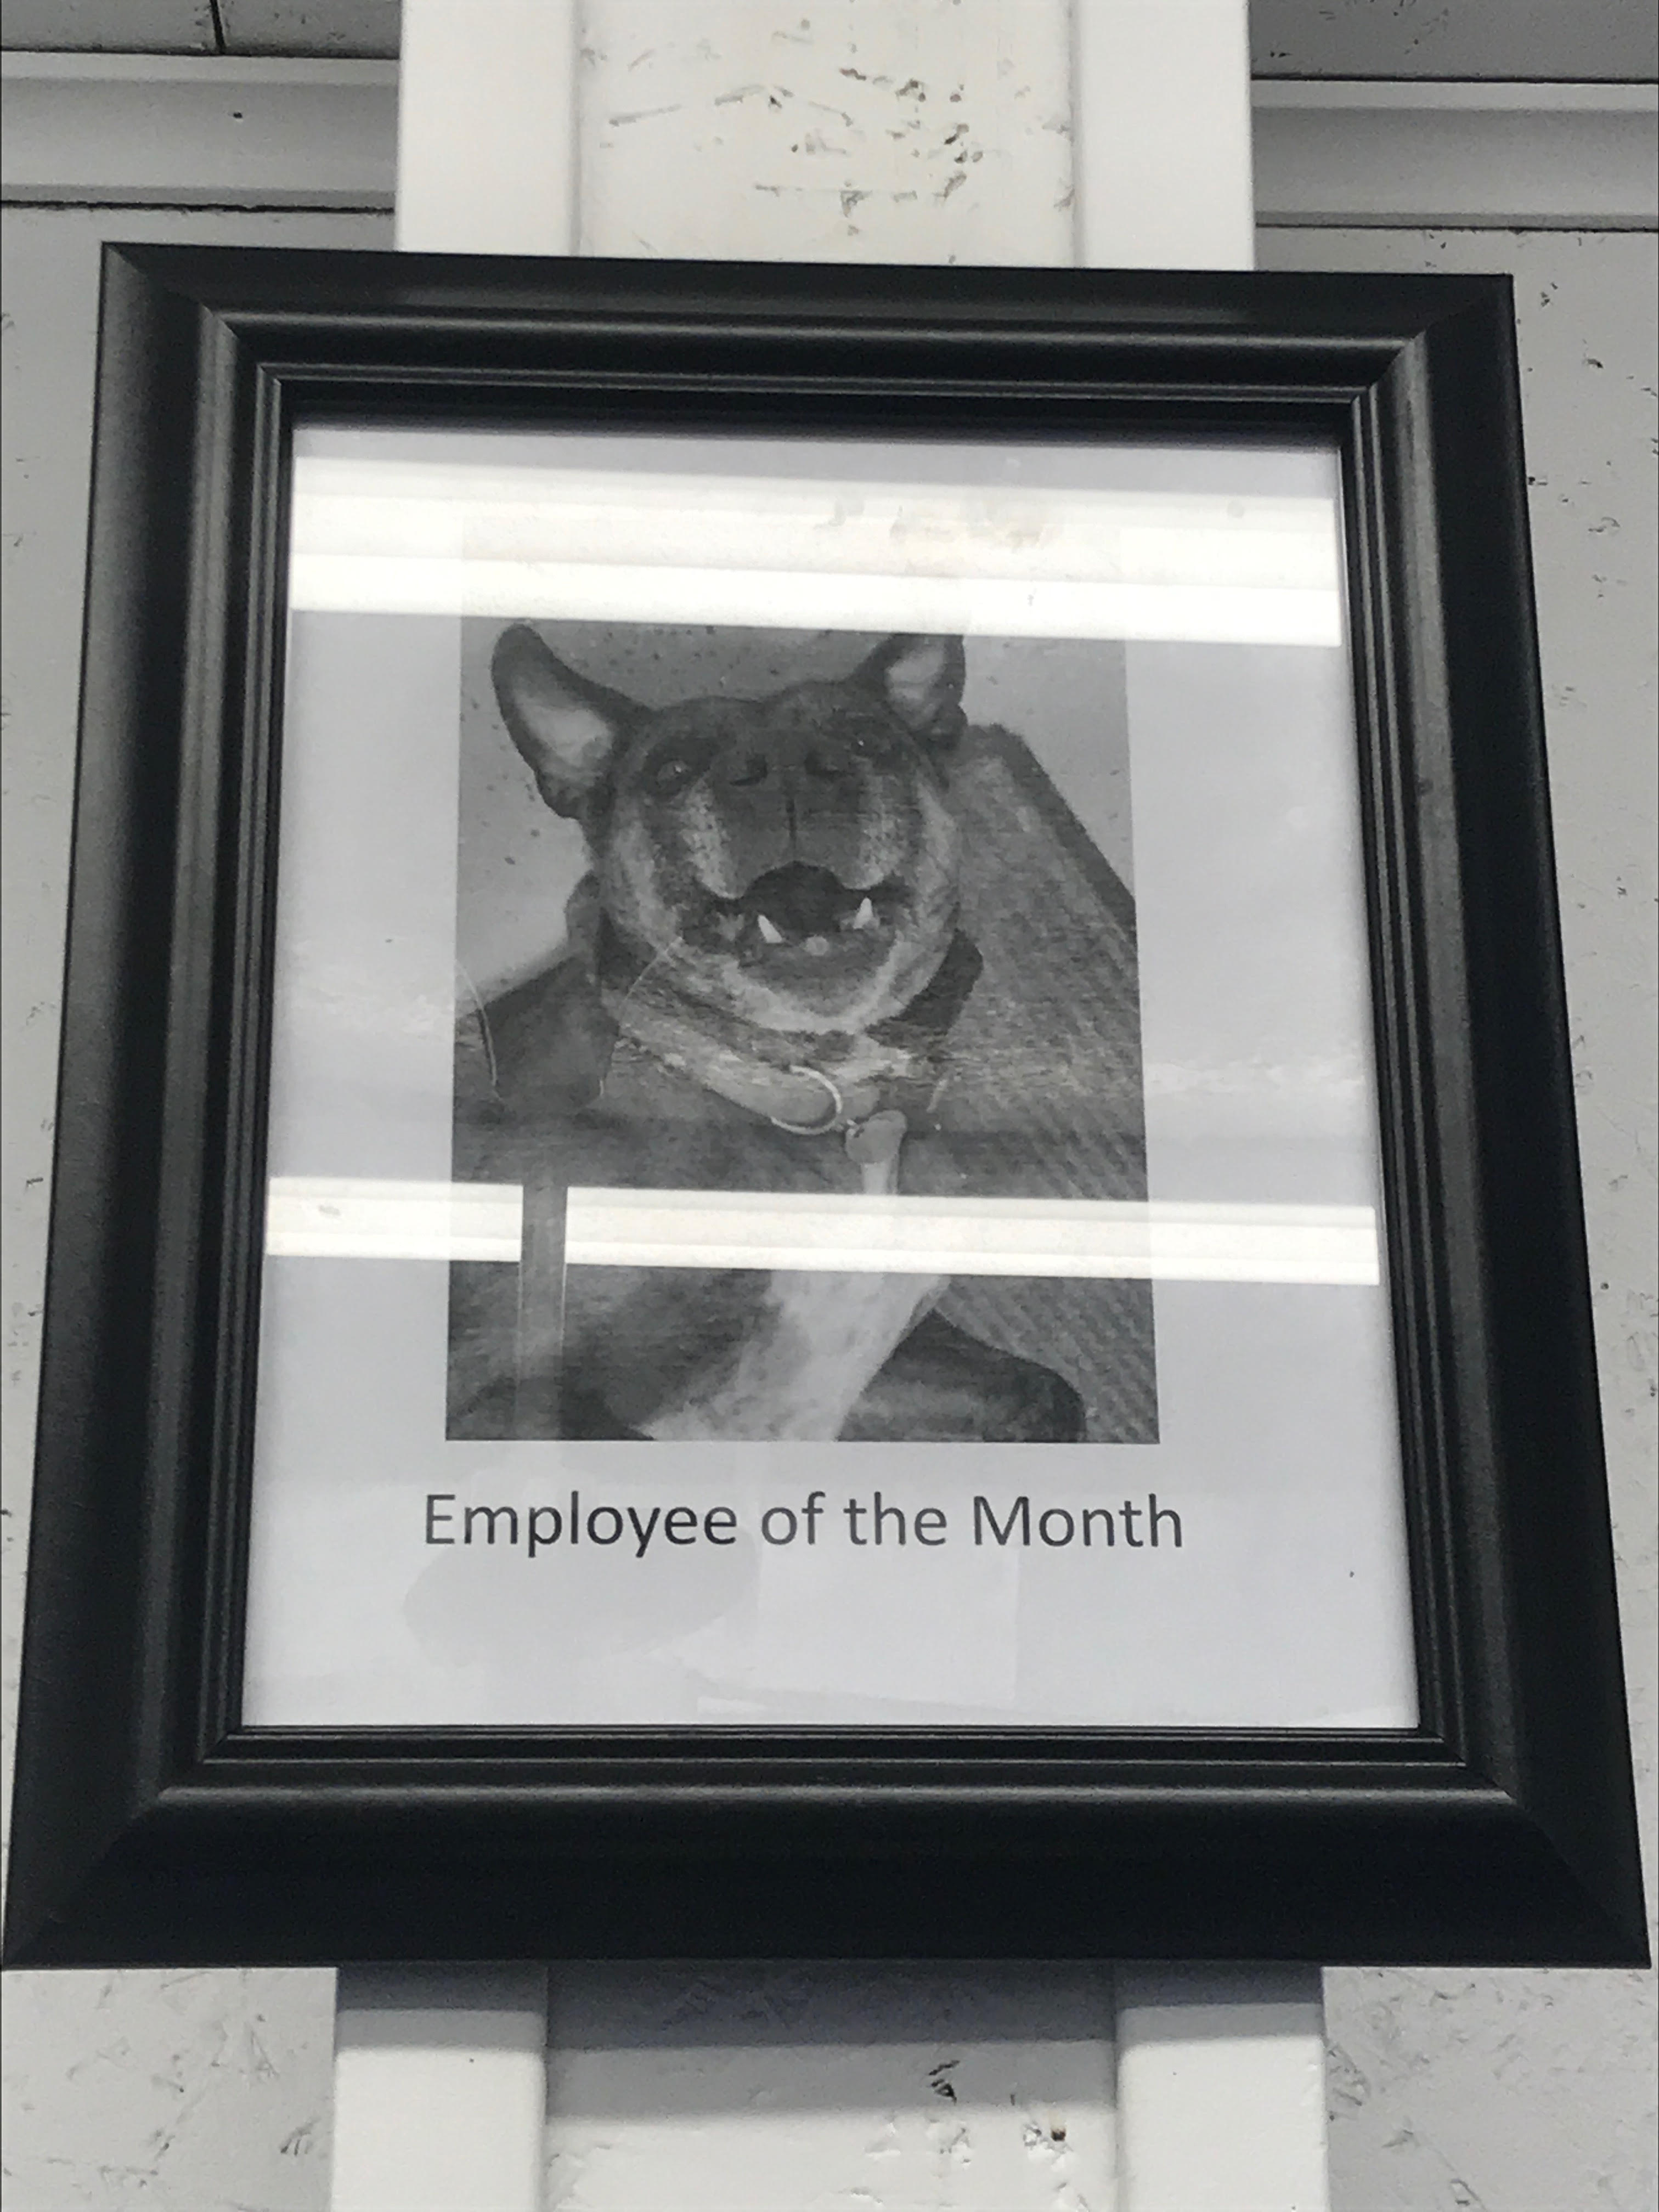
\includegraphics[width=0.5\linewidth]{
   Month.jpg} % first figure
        \caption{Macy}
    \end{minipage}\hfill
    \begin{minipage}{0.45\textwidth}
      \centering
      
\includegraphics[width=0.5\linewidth]{
   BlockI-Logo-Full-Color-CMYK.jpg} % second figure
    \end{minipage}
    \end{figure}
\end{frame}

% SLIDE (FINAL SLIDE)------------------------
\begin{frame}
\Huge{\centerline{The End}}
\end{frame}

%------------------------------------------------
\end{document}
